\section{Main Services}
\label{sec:main_services}
The next sections explain the idea of the three main services of the Basilisk platform, namely \acf{hcs} (section \ref{sec:hooks_checking_service}), \acf{jms} (section \ref{sec:jobs_managing_service}), and \acf{tbs} (section \ref{sec:ts_benchmarking_service}).

This explanation follows the flow of actions that happen while a user configures a continuous benchmark and the process that happens when a benchmark is initiated. This is based on code review and analysis and information and diagrams provided by former developers of the project.
\\

Figure \ref{fig:basilisk_high_level_design_approach} gives an overview of the three microservices of the Basilisk platform.
It shows the most essential messages sent between the services and the interactions with \gh{} and \dockh{}.
Messages sent between the services are sent using a RabbitMQ message broker.
The users interact with the services through REST endpoints which are not shown in this figure.
Interactions of the users with the REST APIs are stateless HTTP requests.
The services and the messages will be explained in the following sections.

\begin{figure}[tbph]
	\centering
	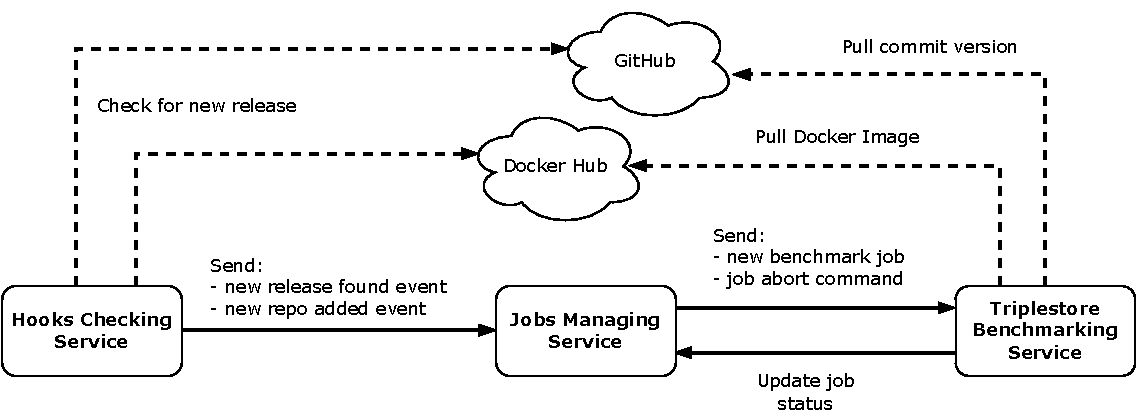
\includegraphics[width=1\textwidth]{figures/high-level-design-approach.pdf}
	\caption{Overview of the three microservices}
	\label{fig:basilisk_high_level_design_approach}
\end{figure}



\subsection{\acl{hcs}}
\label{sec:hooks_checking_service}
The main task of the \ac{hcs} is to observe \gh{} and \dockh{} repositories of \tsp{} for new releases or changes.

When a user wants to set up a new continuous benchmark, a \ts{} is registered at the \ac{hcs} by defining the repository (\gh{} or \dockh{}) that has to be observed for changes.
This happens through REST API calls to the \ac{hcs} providing the repository's name and owner.
The \ac{hcs} will then create a hook for the repository to get noticed about changes.
In general, a hook is a piece of code or software that attaches itself to a software component to intercept messages and react to those messages, \eg, with function calls.
In the case of the \ac{hcs} the hooks can be seen as bookmarks for the repositories.
Each hook stores the latest known version of a repository.
The service will query the saved repositories regularly by polling the REST APIs of \gh{} and \dockh{} and compare their current version to the version stored in the hook.

When the \ac{hcs} notices a new release for a repository, it updates the corresponding hook to the newest version.
Then it sends a message about the new version to the \aclp{jrq} from which the \acl{jms} retrieves the message.

\subsubsection{API and Messaging}
\label{sec:hooks_api}
The \ac{hcs} is controlled by the user over a REST API.

The continuous checking of the repositories can be started and stopped over a REST endpoint.
The other endpoints are for adding and deleting \gh{} and \dockh{} repositories.
Figure \ref{fig:rest_apis_approach_hcs} shows these endpoints.
\begin{figure}[tbph]
	\centering
	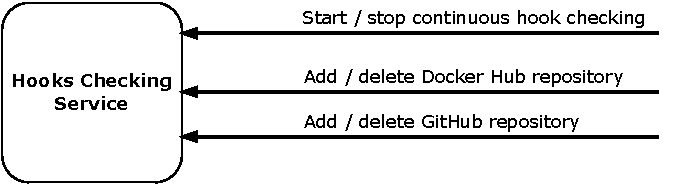
\includegraphics[width=.57\textwidth]{figures/rest-apis-approach-hcs.pdf}
	\caption{REST API of the \acl{hcs}}
	\label{fig:rest_apis_approach_hcs}
\end{figure}

The communication between the \ac{hcs} and the \acl{jms} is done with RabbitMQ (\ref{sec:rabbitmq}) messages, by using the \aclp{jrq}.
The messages contain different events that can occur in the \ac{hcs}.
For example, an event is sent when adding or deleting a repository, or a new release is detected.


\subsection{\acl{jms}}
\label{sec:jobs_managing_service}
The \acf{jms} has two core functions: first, it manages configurations of \tsp{}.
These are used for their second function, creating and managing benchmarks jobs.
Lastly, the \ac{jms} manages the status for running and pending jobs sent to the \ac{tbs}.
\\

There are three configuration types needed for a benchmark job.
First, the platform needs the configuration for the \ts{}.
This configuration\footnote{\url{http://iguana-benchmark.eu/docs/3.2/usage/configuration/}} includes, for example, the SPARQL endpoint as well as the user and password for the connection to the endpoint.
The \iguana{} framework needs these arguments to properly connect to the \ts{} under test.

Secondly, the platform needs configurations for datasets and query files.
The dataset configuration consists of the dataset name and the URL for the dataset's location on the server.
The query configuration consists similarly of a name for the queries and the URL for the location of the query file.

All of the named configurations are managed over the REST API of the \ac{jms}.
\\

When the \ac{jms} receives an event from the HCS regarding a new release of a repository, the \ac{jms} will create benchmark jobs for the new release.
A benchmark job consists of the current version of the repository, a query configuration, and a dataset.
For each event, multiple benchmark jobs are created.
Each benchmark job has a query file and a dataset that is used for the benchmark.

These benchmark jobs will then be sent to the \ac{tbs} over the \acl{bjq}.

The management of the running and pending benchmark jobs is done by the REST API of the \ac{jms}.
When an endpoint is triggered, \eg, to abort a pending job, the \ac{jms} sends an event to the \ac{tbs}.


\subsubsection{API and Messaging}
\label{sec:jobs_api}
The \ac{jms} communicates with the \ac{hcs} and the \ac{tbs} over RabbitMQ message queues.
Repository events are received from the \ac{hcs} and benchmark job events are send to the \ac{tbs} over the \ac{bjq}.
\\

Interaction with the user is handled over the REST API.
The API offers endpoints for adding and deleting the different configurations of \tsp{}, datasets, and queries.
The second set of endpoints are for querying the job status of running and pending jobs and for stopping individual jobs.
Figure \ref{fig:rest_apis_approach_jms} shows these endpoints.
\begin{figure}[tbph]
	\centering
	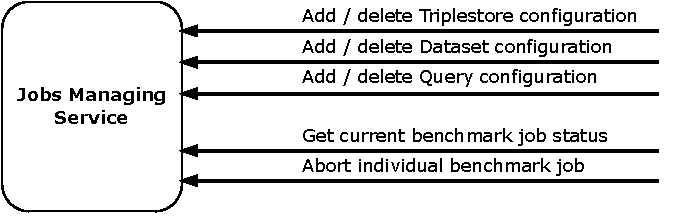
\includegraphics[width=.57\textwidth]{figures/rest-apis-approach-jms.pdf}
	\caption{REST API of the \acl{jms}}
	\label{fig:rest_apis_approach_jms}
\end{figure}


\subsection{\acl{tbs}}
\label{sec:ts_benchmarking_service}
The \acf{tbs} executes the benchmark jobs it receives from the \ac{jms} and saves the benchmarking results to the \acl*{jsts}.

To execute a benchmark, the service needs a running instance of the \ts{} with the loaded dataset on which the benchmark will be executed.
This instance is built from the information and configurations provided in the benchmark job.
The \ac{tbs} will query the provided repository (\gh{} or \dockh{}) for the version specified in the job.

If the repository is from \gh{}, the \ac{tbs} downloads the source code for the provided commit and searches for a Dockerfile.
The service then builds and runs a Docker container from that Dockerfile.

If the repository is from \dockh{}, the \ac{tbs} pulls the image with the provided tag.
The service then runs the image as a Docker Container.

Loading the dataset depends on the \ts{}.
Some \tsp{} like \tentris{}\footnote{\url{https://tentris.dice-research.org/}} can load a dataset on startup.
Other \tsp{} like Oxigraph\footnote{\url{https://github.com/oxigraph/oxigraph}} require the dataset to be loaded through a REST endpoint after the \ts{} is started.
\\

After starting the Docker Container, the \ac{tbs} creates a configuration file for the \iguana{} framework.
\iguana{} will then perform the benchmark with the provided configurations.

When the benchmark is finished, the results are written to the \acf{jsts}.

\subsubsection{API and Messaging}
\label{sec:benchmarking_api}
The \ac{tbs} has no REST API.
The service is controlled through the \ac{jms} by events send over RabbitMQ.

The events received from the \ac{jms} are new benchmark jobs and pause or abort commands for running benchmark jobs.
The \ac{tbs} sends short events containing the status of benchmark jobs, \eg, a job has started or it has finished, and the results are uploaded to the \acl{jsts}.